\section{Fallender Schnee}

\subsection{Hintergründe}

Schnee ist, genau wie Regen, eine Spezialform von \PimiddyBegriff{Niederschlag}.
Hier soll kurz auf die Entstehung von Niederschlag und die Bildung von
Schneeflocken eingegangen werden. Der Erklärungsansatz orientiert sich
an \cite{wiki:Luftfeuchtigkeit}.

Überall dort, wo sich eine freie Wasseroberfläche wie z.\,B.\ ein See befindet und
die Temparatur einen bestimmten Wert übersteigt, lösen sich Moleküle der
Wasseroberfläche von ihrem Verbund und verdunsten in die Luft. Umgekehrt treffen
verdunstete Wassermoleküle wieder auf die Wasseroberfläche und kondensieren
dort. Die \emph{Kondensationsrate} und die
\emph{Verdunstungsrate} geben an, wie viel Wasser in einem Bereich zu
einem Zeitpunkt verdunstet und wie viel kondensiert.

Stellt man sich eine Wasseroberfläche bei trockener Luft vor, so ist
die Kondensationsrate anfangs 0, da keine Wassermoleküle in der Luft
enthalten sind, die kondensieren können. Die Verdunstungsrate ist
bei einer ausreichend hohen Temperatur allerdings ungleich 0. Mit der
Zeit steigt so die Anzahl der Wassermoleküle in der Luft, die Luft
\PimiddyQuotes{sättigt} sich mit Wasser. Dadurch steigt widerum die
Kondensationsrate. Bei gleich bleibenden Bedingungen gleichen sich
nach einiger Zeit die Kondensation und Verdunstung aneinander an.  Die
in diesem Gleichgewichtszustand vorliegende Konzentration von
Wassermolekülen in der Luft ist die
\PimiddyBegriff{Sättigungskonzentration} oder \PimiddyBegriff{maximale
Luftfeuchtigkeit}. Sie ist umso höher, je wärmer es ist, siehe
\autoref{fig:implementation_moist_air}. Umgangssprachlich sagt man
daher, warme Luft könne \PimiddyQuotes{mehr Wasser aufnehmen}.

\begin{figure}[ht]
\centering
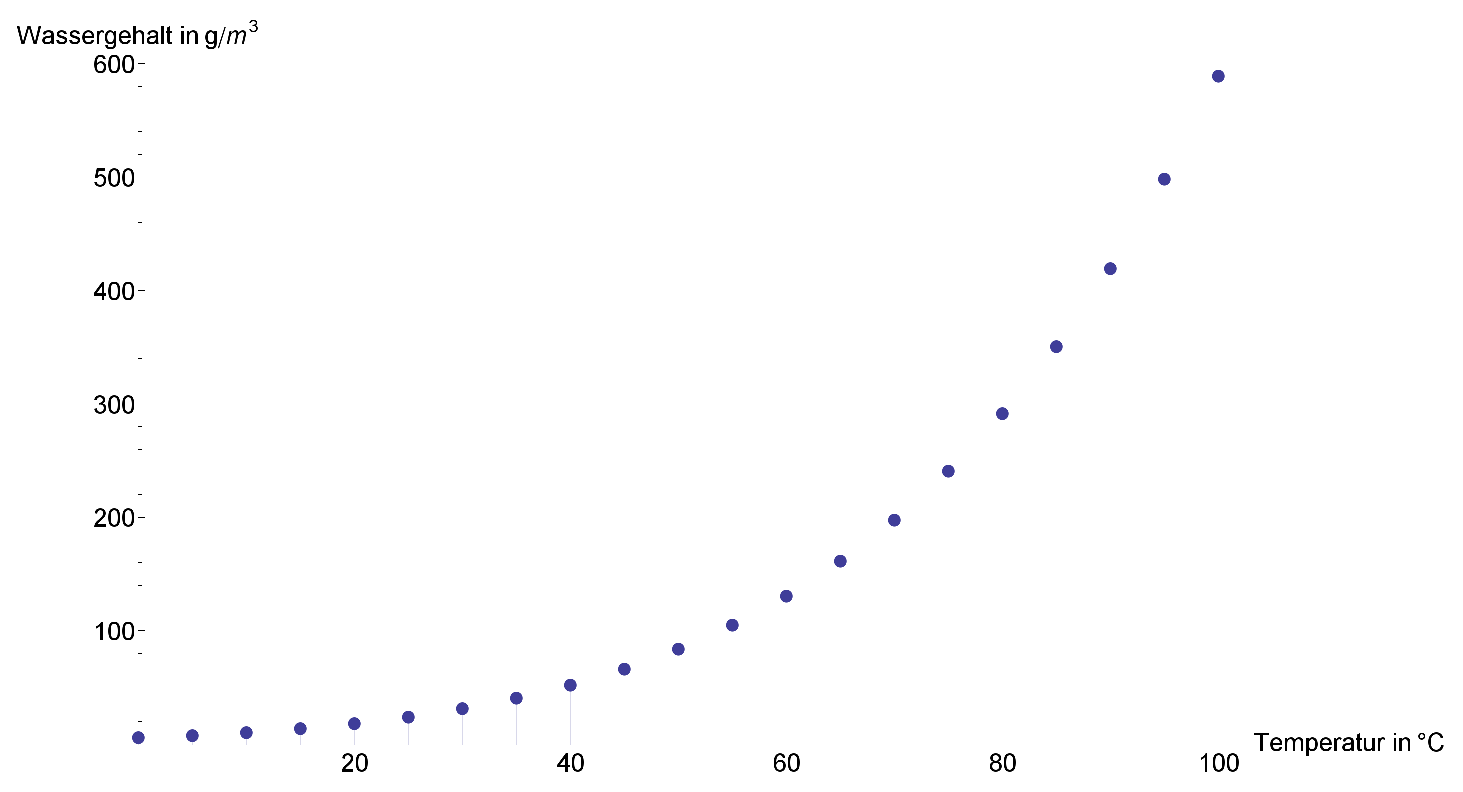
\includegraphics[width=10cm]{images/moist_air}
\caption{Der exponentielle Zusammenhang zwischen Temperatur und Sättigungsmenge von Wasserdampf in der Luft. (Artikel Sättigung (Physik) in Wikipedia, das nochmal ggf. mit matlab nachplotten)}
\label{fig:implementation_moist_air}
\end{figure}

Steigt warme Luft mit hoher Wassersättigung vom Boden in die
Atmosphäre auf, kann die Sättigungsmenge in den höheren Luftschichten
über den eigentlich maximalen Wert steigen -- es entsteht wieder ein
Ungleichgewicht. Um dieses Ungleichgewicht zu kompensieren, kondensiert
das überschüssige Wasser an sogenannten
\PimiddyBegriff{Kondensationskernen} (beispielsweise Staubpartikeln in
der Luft) und es bilden sich kleine Wassertröpfchen in
Mikrometergröße. Passiert dies großflächig, entstehen Wolken am
Himmel. Verdichten sich die kondensierten Tropfen weiter, werden sie
irgendwann zu schwer und fallen aufgrund der Schwerkraft herunter, es
entsteht \emph{Regen}.

Eine Spezialform der eben beschriebenen Kondensationskerne sind die
\emph{Kristallisationskerne}. Bei Temperaturen unter \PimiddyDegree{0}
bilden sich an diesen Kernen keine Tropfen sondern \emph{Kristalle}.
Bei starken Minustemperaturen (ab \PimiddyDegree{-40}) müssen sie
jedoch nicht vorhanden sein, es bildet sich auch so Kristalle.

Diese Kristalle sind anfangs noch sehr klein, sie wachsen erst während ihres
Falles zu Boden weiter an. Dabei entstehen aufgrund spezieller
Eigenschaften des Wassers charakteristische Formen, siehe
\autoref{fig:implementation_single_snow_crystal}. Durch die Verkettung
mehrerer Kristalle entstehen die Schneeflocken, die man beim
Zubodenfallen beobachten kann. Sie können eine Größe von bis zu 10cm
erreichen\cite{Nau96} und haben ebenfalls vielfältige Formen, die
allerdings keine Symmetrie mehr aufweisen, siehe
\autoref{fig:implementation_real_snowflakes}.

\begin{figure}
    \begin{subfigure}[b]{0.5\textwidth}
            \centering
            \includegraphics[width=\textwidth]{images/single_snow_crystal}
            \caption{Ein einzelner \PimiddyQuotes{farn-artiger} Schneekristall\cite{Yanagi2011}.}
            \label{fig:implementation_single_snow_crystal}
    \end{subfigure}
    ~
    \begin{subfigure}[b]{0.5\textwidth}
            \centering
            \includegraphics[width=\textwidth]{images/real_snowflakes}
            \caption{Kameraaufnahmen einzelner Schneeflocken mit etwa 1-2cm Durchmesser\cite{Hanesch1966}.}
            \label{fig:implementation_real_snowflakes}
    \end{subfigure}
\end{figure}

\begin{figure}[ht]
\centering
\includegraphics[width=8cm]{images/snowflake_size_graph}
\caption{Der Zusammenhang von Schneeflockengröße und Temparatur nach \cite{Jun00}.}
\label{fig:implementation_snowflake_size_graph}
\end{figure}

\subsection{Visualisierung}

Bei der Wahl der Visualisierungsmethode müssen mehrere Faktoren in
Betracht gezogen werden. Die Simulation soll sowohl ruhige
Wetterverhältnisse mit wenigen Schneeflocken als auch Szenen mit
starkem Wind und sehr vielen Schneeflocken behandeln können. Daher ist
einerseits wichtig, dass einzelne Schneeflocken einen gewissen
Detailgrad besitzen, aber die Performance gleichzeitig so wenig wie
möglich beeinträchtigen.

Es sollen mindestens die zwei wichtigsten Eigenschaften einer
Schneeflocke modelliert werden: die Größe und das Aussehen. Beide
Eigenschaften hängen von der Umgebungstemparatur ab. Für den Durchmesser $D$
einer Schneeflocke in Abhängigkeit von der Temperatur $T$ wurde in
\cite{Jun00} folgende Relation aufgestellt (siehe
\autoref{fig:implementation_snowflake_size_graph}):

\begin{equation}
\label{eq:implementation_snowflake_diameter}
D =
\begin{cases}
0.015 \cdot |T|^{-0.35} & \PimiddyFormelText{ für }T \leq -0.061 \\
0.04 & \PimiddyFormelText{ für }T > -0.061
\end{cases}
\end{equation}

Das Aussehen einer Schneeflocke bestimmt sich primär dadurch, ob
\emph{trockener} oder \emph{feuchter} Schnee vorliegt. Nahe bei
\PimiddyDegree{0} ist der Schnee feucht und hat eine hohe
Dichte. Bei kälteren Temperaturen werden die Schneeflocken kleiner und
sehen zarter aus.

Aagaard hat in \cite{Aagaard2004} ein Modell entwickelt, welches die
tatsächliche Form der Schneeflocke abhängig von Dichte und Größe
möglichst genau abbildet. Dazu verwendet er zufällig generierte, weiß
gefüllte Dreiecke, welche die Eiskristalle darstellen sollen. Anhand
des (randomisierten) Durchmessers der Schneeflocke wird eine Anzahl
von \emph{Schichten} ermittelt, in der die Dreiecke dann angeordnet werden,
siehe \autoref{fig:implementation_aagaard_layer_model} und
\autoref{fig:implementation_aagaard_spheres}. Auf diese Art können
vielfältige zufällige Formen generiert und an die aktuellen
Wetterbedingungen angepasst werden. Durch die dreidimensionale
Modellierung kann man den Flocken außerdem eine Rotation geben und sie
von allen Seiten betrachten.

Allerdings ist das Modell sehr laufzeitintensiv. Dies hat zwei Ursachen:

\begin{enumerate}
\item Die einzelnen Dreiecke einer Schneeflocke sind
halbtransparent. Dies führt dazu, dass weit mehr Fragments erzeugt
werden als es Pixel auf dem Bildschirm gibt. Diesen Effekt nennt man
\emph{Overdraw}.
\item Es werden Außerdem sehr sehr viele kleine Dreiecke für eine einzelne
Flocke benötigt (Aagaard geht von mindestens 10 aus, maximal über
100). Für 1.000 Flocken erhält man so schon 10.000 Dreiecke. Die
angestrebte Flockenzahl bei heftigem Schneefall liegt aber bei weit
über 1.000 Flocken. Aagaard schlägt daher vor, ein \PimiddyQuotes{Level
of detail}-System einzubauen, bei dem weiter entfernte Flocken durch
simplere Geometrie (z.\,B.\ mit weniger Dreiecken) angenähert werden. Er
implementiert dies jedoch selber nicht, da Performance kein
entscheidender Faktor für die Implementierung ist.
\item Die Eigenschaften einer Schneeflocke wie etwa ihre Geschwindigkeit
und die Darstellung der Flocke müssen getrennt werden, da OpenGL es
nicht direkt erlaubt, Daten für einen \PimiddyQuotes{Block} von
Primitiven anzugeben wie etwa die Dreiecke der Schneeflocke. Dies
macht die Implementierung schwieriger und langsamer.
\end{enumerate}

\begin{figure}[ht]
    \centering
    \includegraphics{images/aagaard_layer_model}
    \caption{Das Resultat von Aagaards 3D-Modell für die Schneeflocken.}
    \label{fig:implementation_aagaard_layer_model}
\end{figure}

\begin{figure}[ht]
    \centering
    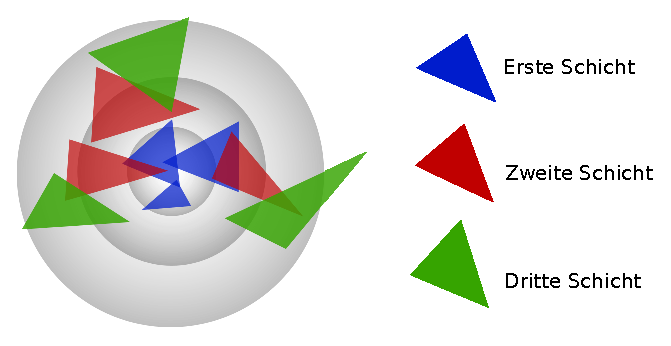
\includegraphics{images/aagaard_spheres}
    \caption{Der schichtweise Aufbau einer Schneeflocke in Aagaards Modell.}
    \label{fig:implementation_aagaard_spheres}
\end{figure}

\begin{figure}[ht]
    \centering
    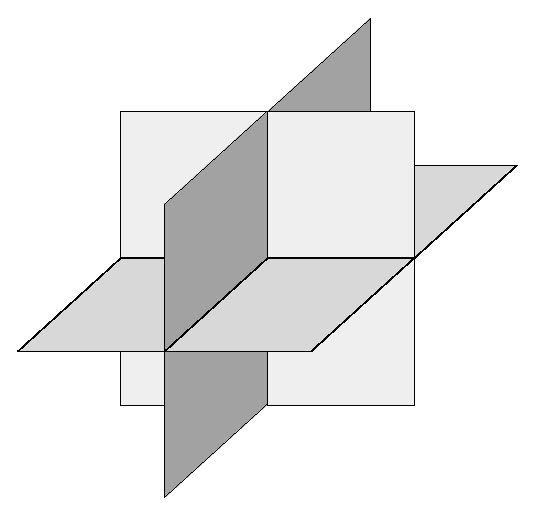
\includegraphics{images/snowflake_three_rectangles}
    \caption{Eine Schneeflocke aus drei Rechtecken zusammengesetzt.}
    \label{fig:implementation_snowflake_three_rectangles}
\end{figure}

In \cite{Saltvik2006} findet sich ein etwas simplerer Ansatz, der nur
drei transparente Rechtecke pro Schneeflocke verwendet (siehe
\autoref{fig:implementation_snowflake_three_rectangles}). Dadurch wird
massiv Performance gespart, die Daten für die Flocken müssen
allerdings trotzdem in einem separaten Buffer gespeichert werden.

In dieser Arbeit wird stattdessen eine simplere Visualisierung mit
Hilfe von sogenannten \PimiddyBegriff{Pointsprites} gewählt. Statt
mehrerer Dreiecke repräsentiert nur ein einzelner Punkt eine
Schneeflocke. Dadurch wird es möglich, alle Daten für eine Flocke im
OpenGL-Buffer selber zu speichern. Zudem sind Punkte in OpenGL sind
allerdings mathematischen Punkte, denn sie besitzen eine
\emph{Ausdehnung}. Dadurch wird es möglich, die Flockengröße zu variieren.

Diese Ausdehnung jedoch nicht in Weltkoordinaten angegeben, sondern in
Pixeln auf dem Bildschirm. Das bedeutet, dass die Flocken immer zum
Betrachter zeigen, man kann sich nicht um sie herum bewegen (siehe
\autoref{fig:implementation_point_sprite_vs_billboard}). Außerdem muss
-- im Gegensatz zu Dreiecken -- eine Formel für die Größe erdacht
werden, damit weiter entfernte Punkte kleiner werden (für Dreiecke
wird dies mit Hilfe einer perspektivischen Projektionsmatrix
sichergestellt).

\begin{figure}[ht]
    \centering
    \includegraphics{images/point_sprite_vs_billboard}
    \caption{Links ein Schneekristall aus zwei Dreiecken zusammengesetzt, rechts als Pointsprite.}
    \label{fig:implementation_point_sprite_vs_billboard}
\end{figure}

\begin{listing}
\begin{minted}{glsl}
uniform mat4 model_view_projection;
uniform vec4 eye_position;

in vec4 position;
in float point_size;

float determine_point_size(float distance_to_camera)
{
   // ...
}

void main()
{
  float distance_to_camera = distance(eye_position,position);
  gl_PointSize = determine_point_size(distance_to_camera);
  gl_Position = model_view_projection * position;
}
\end{minted}
\caption{Der zu Pointsprites gehörige Vertexshader}
\label{lst:implementation_point_sprite_vertex_shader}
\end{listing}

\begin{listing}
\begin{minted}{glsl}
uniform sampler2D snowflake_texture;

out vec4 fragment_color;

void main()
{
  // Einfarbige Punkte (hier weiss)
  // fragment_color = vec4(1.0,1.0,1.0,1.0);
  // Mit Textur:
  fragment_color = texture(snowflake_texture,gl_FragCoord);
}
\end{minted}
\caption{Der zu Pointsprites gehörige Fragmentshader}
\label{lst:implementation_point_sprite_fragment_shader}
\end{listing}

Um Pointsprites in OpenGL zu zeichnen, gibt man bei der OpenGL-Funktion
\PimiddyInlineCode{glDrawArrays} den Primitvtyp
\PimiddyInlineCode{GL\_POINTS}
an. \PimiddyListingRef{lst:implementation_point_sprite_vertex_shader}
zeigt den dazugehörigen Vertexshader, der als Input die
Projektionsmatrix, den Augenpunkt, die Größe der Schneeflocke und
deren Position bekommt. Mit Hilfe der Variable
\PimiddyInlineCode{gl\_PointSize}, der man einen
\PimiddyInlineCode{float}-Wert zuweist, kann man die Größe des Punktes
setzen. Die Funktion \PimiddyInlineCode{determine\_point\_size} wird
gleich erläutert.

Der zu
\PimiddyListingRef{lst:implementation_point_sprite_vertex_shader}
gehörige Fragmentshader
\PimiddyListingRef{lst:implementation_point_sprite_fragment_shader}
verwendet den zweidimensionalen Vektor
\PimiddyInlineCode{gl\_FragCoords} $\in [0,1]^2$. Dieser Vektor gibt
an, wo sich das Fragment innerhalb des aktuellen Punktes (respektive,
der aktuellen Flocke) befindet. OpenGL verwaltet also ein eigenes
Koordinatensystem innerhalb des Punktes. Mit Hilfe dessen kann man den
Punkten im Fragmentshader nicht nur eine einheitliche Farbe geben,
sondern auch eine Textur. Die Textur der Punkte wird in der
Implementierung zufällig aus einer Menge von Texturen ausgewählt, die
zur aktuellen Außentemperatur passen.

Um den Vertexshader zu komplettieren, muss noch die Größe der
Pointsprites bestimmt werden. Verwendet man für seine Szene eine
perspektivische Projektion, besteht zwischen dem Abstand von Objekten
und ihrer dargestellten Größe ein nichtlinearer Zusammenhang. Daher
sollte auch für die Größe der Pointsprites eine ähnliche
Proportionalität bestehen. Microsofts DirectX-Framework verwendet
hierfür folgende
Formel\cite{DirectXPointSprites}:

\begin{equation}
\label{eq:implementation_snowflake_perspective_formula}
S =
S'
\sqrt{
  \frac
  {
    1
  }
  {
    A +
    B \cdot D_e +
    C \cdot D_e^2
  }
}
\end{equation}

$S'$ bezeichnet hierbei die vorgegebene Punktgröße, die Konstanten
$A,B,C$ sind frei wählbar und $D_e$ bezeichnet den Abstand des Punktes
von der Kamera. Die Werte $A=0.96,B=0.19,C=0.06$ haben sich als
visuell ansprechend herausgestellt.

Für die Simulation von heftigem Schneefall reicht es allerdings nicht
aus, nur die Anzahl der Flocken zu erhöhen und deren Größe zu
randomisieren. Das menschliche Auge interpretiert die Flocken dann
eher als unrealistisches \PimiddyQuotes{Rauschen}. Um dies auszumerzen
wird in \cite{Langer2004} wird ein Verfahren vorgestellt, mit dem in
der Bildebene aus einigen wenigen Schneeflocken weitere synthetisiert
werden, sodass ein realistischer Eindruck einer großen Menge
Schneeflocken entsteht. Dieses Verfahren ist sehr performant,
allerdings relativ schwierig umzusetzen. Daher wurde ein anderer Weg
gewählt, nämlich die \emph{Transparenz} der Schneeflocken ebenfalls
abhängig von der Entfernung zur Kamera mit Hilfe von
\autoref{eq:implementation_snowflake_perspective_formula} zu
variieren, allerdings mit den Konstanten $A=0.1,B=0.15,C=0$ und
$S'=1$.

Mit Hilfe von Pointsprites ist es möglich, auf einem aktuellen System
weit über 100.000 Schneeflocken gleichzeitig anzuzeigen. Es ist jedoch
nicht möglich, die Flocken rotieren zu lassen, was allerdings visuell
nicht kritisch ist.

\subsection{Modellierung}

\subsubsection{Einleitung}

Nach der visuellen Beschreibung der Schneeflocken soll nun deren
Bewegung erläutert werden. Dazu wird zuerst ein physikalisch
motiviertes Modell eingeführt und danach die Implementierungsdetails
des Partikelsystems erklärt.

Physikalisch gesehen ist eine Schneeflocke ein \emph{Körper} mit einer
sehr geringen Masse. Kennt man die aktuelle Geschwindigkeit $\vec{v}$
des Körpers, sowie seine momentane Position $\vec{p}$ und hat man ein
Zeitdelta $\Delta t$ gegeben, dann kann seine Bahn $\vec{s}$ in diesem
Zeitschritt durch das \emph{Weg-Zeit-Gesetz} bestimmt werden, sofern
man die momentane Beschleunigung $\vec{a}$ kennt:

\begin{equation}
\label{eq:implementation_snowflake_path_time_law}
\vec{s} = \frac{1}{2} \vec{a} \Delta t^2 + \vec{v}t + \vec{p}
\end{equation}

Dabei nimmt man natürlich an, die Beschleunigung sei in dem
Zeitabschnitt $\Delta t$, den man grade betrachtet, konstant. Für die
Beschleunigung selber gilt Newtons Formel:

\begin{gather}
\vec{F} = m \cdot \vec{a} \\
\vec{a} = \frac{\vec{F}}{m}
\end{gather}

Man muss also -- wie schon beim Windfeld -- berechnen, welche Kräfte
auf die Schneeflocke wirken. Daraus ergibt sich dann die Flugbahn. Es
bietet sich manchmal auch an, eine Kraft nicht als Beschleunigung zu
modellieren, sondern sie in
\autoref{eq:implementation_snowflake_path_time_law} direkt auf die
Geschwindigkeit zu addieren (die Geschwindigkeit der Schneeflocke also
unangetastet zu lassen). Im Folgenden sollen die einzelnen Kräfte
näher beleuchtet werden.

In \cite{Aagaard2004} wurden vier Kräfte zusammengetragen, welche
zusammen die Bewegung einer Schneeflocke beeinflussen:

\begin{enumerate}
\item Die Schwerkraft $\vec{F}_g$ ist eine konstante Kraft, die
-- genau wie beim Windfeld -- in negativer $y$-Richtung wirkt.
\item Der Wind übt eine Kraft $\vec{F}_\PimiddyFormelText{w}$
auf die Schneeflocke aus, die den \PimiddyBegriff{Luftwiderstand}
widerspiegelt. Aufgrund der niedrigen Dichte ist dies die Kraft,
welche die Flocke am meisten in ihrer Bahn beeinflusst.
\item Die aerodynamische Form der Flocke führt dazu, dass sie selbst bei
Windstille keine direkte Bahn nach unten verfolgt, sondern in kleinen
Spiralbahnen zur Erde fällt. Dieser Effekt wird
\PimiddyBegriff{dynamischer Auftrieb} genannt. Er wird jedoch nicht
als Kraft modelliert, sondern direkt als Geschwindkeit (siehe unten).
\item Auch Schneeflocken haben einen gewissen \emph{statischen
Auftrieb} $F_{\PimiddyFormelText{Auftrieb}}$ innerhalb der umgebenden
Luft.
\end{enumerate}

Diese Kräfte werden nun einzeln besprochen.

\subsubsection{Luftwiderstand}

Die Methode von Stam liefert ein dreidimensionales Vektorfeld von
Geschwindigkeiten. Das bedeutet, man kann in jedem Punkt innerhalb der
Simulationsgrenzen eine Windgeschwindigkeit angeben (wenn der Punkt
nicht auf dem Gitter liegt, wird stattdessen ein Geschwindigkeitswert
interpoliert). Es ist aber noch nicht klar, welchen Einfluss die
Windgeschwindigkeit auf die Geschwindigkeit der Flocke ausübt, welche
Kraft also aus der Geschwindigkeit resultiert. Im Folgenden wird eine
einzelne Schneeflocke an Position $\vec{p}_f$ mit Geschwindigkeit
$\vec{v}_{f}$ betrachtet. Mit $\vec{v}_w$ sei die Geschwindigkeit des
Windes an Position $\vec{p}_f$ bezeichnet.

Der Luftwiderstand -- oder allgemeiner der
\PimiddyBegriff{Strömungswiderstand} in Fluiden -- bezeichnet eine
Kraft, die ein Fluid der Bewegung eines Körpers entgegensetzt. Bei der
Berechnung dieser Kraft kommt es auf die \emph{Relativgeschwindigkeit}
von Schneeflocke und Wind an. Herrscht Windstille (ist also $\vec{v}_w
= 0$), sorgt die Schwerkraft für eine konstante Beschleunigung nach
unten, die Flocke fällt mit immer schneller zu Boden. Der
Luftwiderstand wirkt dieser Beschleunigung entgegen, und das umso
stärker, je schneller die Flocke ist. Dadurch stellt sich irgendwann
ein Gleichgewicht zwischen Schwerkraft und Luftwiderstand ein und die
Flocke erreicht ihre \PimiddyBegriff{Endgeschwindigkeit}
$v_{y,\PimiddyFormelText{max}}$. Im Vakuum hingegen könnte eine
Schneeflocke theoretisch beliebig schnell fallen. $\vec{v}_r$
bezeichne die Relativgeschwindigkeit von Flocke und Wind:

\begin{equation}
\vec{v}_r = \vec{v}_w - \vec{v}_f
\end{equation}

Streng genommen ist der Luftwiderstand aufgeteilt in
\PimiddyBegriff{Druckwiderstand} und
\PimiddyBegriff{Reibungswiderstand}. Deren Anteile hängen von der Form
des umströmten Körpers ab. Bei einer Kreisscheibe überwiegt der
Druckwiderstand, bei einer Tragfläche eines Flugzeugs beispielsweise
der Reibungswiderstand, siehe
\autoref{fig:implementation_snowflake_drag_forces}. Die Unterscheidung
spielt hier aber keine Rolle.

\begin{figure}[ht]
    \centering
    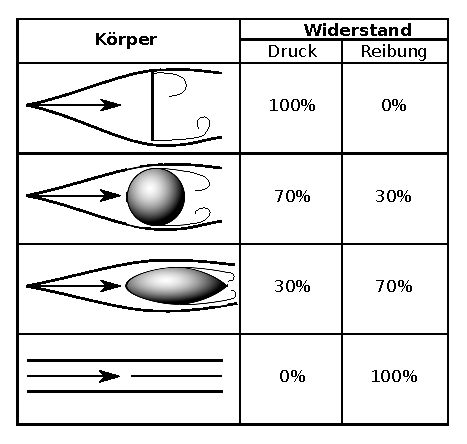
\includegraphics{images/drag_forces}
    \caption{Der Zusammenhang von Druck- und Reibungswiderstand in Abhängigkeit der Form des umströmten Objekts.}
    \label{fig:implementation_snowflake_drag_forces}
\end{figure}

Der Luftwiderstand kann für Fluide mit einer relativ hohen
Geschwindigkeit (die Windgeschwindigkeit fällt in diese Kategorie) mit
der folgenden Luftwiderstandsformel angegeben werden, die auf \PimiddyName{Rayleigh}
zurückgeht:

\begin{equation}
\label{eq:implementation_snowflake_drag_equation}
\vec{F}_w = \frac{1}{2} \rho \vec{v}_r^2 C_d A
\end{equation}

In der Formel bezeichnet $\rho$ die Dichte der Luft, die bei
\PimiddyDegree{0} etwa $1.293\frac{kg}{m^3}$ beträgt. $A$ bezeichnet
die \emph{Bezugsfläche} des Körpers, den man betrachtet. Nähert man
die Schneeflocke als Kugel mit Radius $r$ an, so kann $A$ als $\pi
r^2$ gewählt werden, wenn man die Projektion der Kugel auf die Ebene
als Referenz wählt, oder $2\pi r^2$, wenn man die
\PimiddyQuotes{Vorderfläche} der Kugel als Refenz wählt. $C_d$
bezeichnet den dimensionslosen
\PimiddyBegriff{Strömungswiderstandkoeffizienten}. Der Luftwiderstand
wächst sich also quadratisch zur Geschwindigkeit des Objekts. Dadurch,
dass die Relativgeschwindigkeit $\vec{v}_r$ in die Formel eingesetzt
wurde, entsteht auch bei Windstille eine zur Geschwindigkeit der
Flocke entgegengesetzte Kraft.

Die Größe $C_d$ ist noch unbekannt. Sie wird normalerweise
experimentell ermittelt. Da zu diesem Thema jedoch keine Ergebnisse zu
finden sind, muss ein anderer Weg gewählt werden, um den Koeffizienten
abschätzen zu können.

Angenommen eine Schneeflocke fällt mit ihrer Endgeschwindigkeit
$v_{y,\PimiddyFormelText{max}}$ grade nach unten. Dann
entspricht die Kraft, die durch den Luftwiderstand hervorgerufen wird,
genau der Schwerkraft:

\begin{align}
\PimiddyBetrag{\vec{F}_g} &= \PimiddyBetrag{\vec{F}_w} \\
m \cdot \PimiddyBetrag{\vec{g}} &= \frac{1}{2} \rho v_{y,\PimiddyFormelText{max}}^2 C_d A
\end{align}

Löst man die untere Gleichung nach $C_d$ auf erhält man:

\begin{equation}
C_d
=
\frac
{
  2 \cdot m \cdot \PimiddyBetrag{\vec{g}}
}
{
  \rho \cdot v_{y,\PimiddyFormelText{max}}^2 \cdot A
}
\end{equation}

Dies eingesetzt in die Luftwiderstandsformel
\ref{eq:implementation_snowflake_drag_equation} ergibt:

\begin{equation}
\vec{F}_w =
\frac
{
  \vec{v}_w^2 \cdot m \cdot \vec{g}
}
{
  v_{y,\PimiddyFormelText{max}}^2
}
\end{equation}

Die Formel hängt nur noch von $v_{y,\PimiddyFormelText{max}}^2$
ab. Diese Größe ist -- im Gegensatz zu $C_d$ -- gut bestimmt worden,
z.B.\ in \cite{Hanesch1966} für Temperaturen zwischen \PimiddyDegree{-2}
und \PimiddyDegree{0}. Dabei wurde festgestellt,
dass die Größe der Schneeflocke kaum Einfluss auf die
Fallgeschwindigkeit hat. Es wurden Geschwindigkeiten im Bereich \PimiddyDegree{0.5}
bis \PimiddyDegree{2.0} gemessen. In
\cite{Centre1998} wurde festgestellt, dass zwischen feuchtem und
trockenen Schnee ein Faktor 2 bezüglich der Geschwindigkeit
besteht. Aaagaard wählt in \cite{Aagaard2004} daher die folgenden
Endgeschwindigkeiten:

\begin{align}
0.5 \frac{m}{s} \leq v_{y,\PimiddyFormelText{max},\PimiddyFormelText{trocken}} \leq 1.5 \frac{m}{s} \\
1 \frac{m}{s} \leq v_{y,\PimiddyFormelText{max},\PimiddyFormelText{feucht}} \leq 2 \frac{m}{s}
\end{align}

Mit Hilfe dieser Formeln lässt ich die Kraft $\vec{F}_w$ für eine
Flocke nun vollständig bestimmen. Wie später erläutert wird, werden
für den Querschnitt $A$ der Flocken, sowie für
$v_{y,\PimiddyFormelText{max}}$ zufällige Werte bestimmt, um ein
natürlicheres Muster zu erzeugen und um die Annäherung der Flocken
durch Kugeln auszugleichen.

\subsubsection{Dynamischer Auftrieb}

Beobachtungen an Schneeflocken bei ruhigem Wetter haben ergeben, dass
die Flocken selten in einer geraden Bahn nach unten fallen, sondern
eher \PimiddyQuotes{Zick-Zack-Bewegungen} machen, siehe
\autoref{fig:implementation_snowflake_helix}.

\begin{figure}[ht]
    \centering
    \includegraphics{images/snowflake_helix}
    \caption{Die ungefähre Bahn eine Schneeflocke ohne den Einfluss von Wind.}
    \label{fig:implementation_snowflake_helix}
\end{figure}

Diese Spiralbahn kann nicht durch den Luftwiderstand hervorgerufen
werden, denn dieser wirkt bei Windstille nur entgegengesetzt der
Schwerkraft, also grade nach oben. Stattdessen wird eine Kraft dadurch
erzeugt, dass sich hinter der Schneeflocke Verwirbelungen bilden und
sie dadurch orthogonal zur Flugbahn ablenken, siehe
\autoref{fig:implementation_snowflake_vortex_shedding}. Dasselbe
Phänomen tritt auch makroskopisch in der Atmosphäre auf, siehe
\autoref{fig:implementation_snowflake_vortex_shedding_macroscopic}.

\begin{figure}[ht]
    \centering
    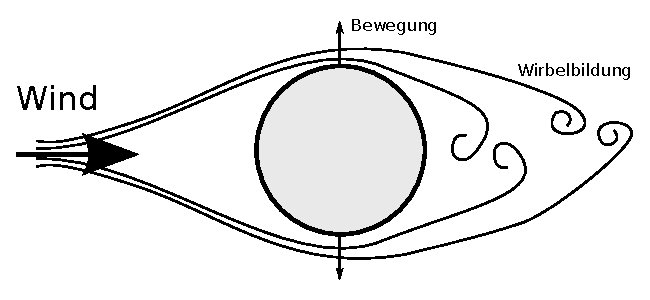
\includegraphics{images/vortex_shedding}
    \caption{Hinter der Schneeflocke bilden sich während des Flugs Wirbel.}
    \label{fig:implementation_snowflake_vortex_shedding}
\end{figure}

\begin{figure}[ht]
    \centering
    \includegraphics{images/vortex_shedding_macroscopic}
    \caption{Die Insel Rishiri-to an der nordwestlichen Küste von Hokkaido, Japan erzeugt Wirbel in der Atmosphäre, die sich über weite Strecken ausbreiten.}
    \label{fig:implementation_snowflake_vortex_shedding_macroscopic}
\end{figure}

Die Wirbel entstehen durch niedrigen Druck, der hinter dem Hindernis
entsteht. Je nach Form des Objekts hat er unterschiedliche
Auswirkungen. Der dynamische Auftrieb auf dünnen, länglichen Objekten
wie den Tragflächen von Flugzeugen sorgt dafür, dass das Flugzeug
abhebt. Er ermöglicht Vögeln und Flugzeugen das Fliegen. Bei stumpfen
Körpern wie Golfbällen oder Schneeflocken hingegen bilden sich die
besagten Wirbel und dadurch eine Seitwärtsbewegung. Diese Wirbel sind
im dreidimensionalen nur sehr schwer zu beschreiben. Statt einem
genauen Modell wird also ein einfacheres Modell angesetzt und der
Effekt nur \PimiddyQuotes{nachgebaut}.

Damit die Schneeflocke sich auf einer kreisförmigen Bahn in der
$xz$-Ebene bewegt, legen wir folgende Ablenkungsgeschwindigkeit zugrunde:

\begin{equation}
\label{eq:implementation_snowflake_lift_velocity}
\vec{v}_{a} =
\omega \cdot r
\left(
\begin{array}{c}
-\sin{\omega t} \\
0 \\
\cos{\omega t}
\end{array}
\right)
\end{equation}

Hier bezeichnet $\omega$ die Winkelgeschwindigkeit, $r$ den
Kreisradius der Bahn und $t$ den Zeitparameter (in diesem Fall kein
Zeitdelta, sondern ein absoluter Wert). Die Flocken sollen allerdings
nur dann eine Kreisbahn einnehmen, wenn ihre Geschwindigkeit relativ
wenig durch den Wind beeinflusst wird. Deshalb wird die
\autoref{eq:implementation_snowflake_lift_velocity} mit einem $C_a$
gewichtet:

\begin{equation}
C_a =
\frac
{
  \PimiddyBetrag{\vec{v}_w - \vec{v}_f}
}
{
  \PimiddyBetrag{\vec{v}_f}
}
\end{equation}

Es wurden keine Experimente bezüglich des Bahnradius $r$ und der
Winkelgeschwindigkeit $\omega$ gefunden. Experimentelle Werte ergeben
aber für diese Größen folgende Einschränkungen:

\begin{gather}
-\frac{\pi}{4} \leq \omega \leq -\frac{\pi}{3} \\
0 \leq r \leq 2
\end{gather}

Auch diese Größen werden also randomisiert.

\subsubsection{Statische Auftrieb}

Wie bereits in \autoref{sec:stam_buoyancy} beschrieben, bezeichnet
Auftrieb eine Kraft, die der Schwerkraft entgegengesetzt ist, wirkt
also in Richtung $(0,1,0)$. Sie entsteht durch die Verdrängung des
Fluids durch einen Körper und sie ist indirekt abhängig von der
Luftdichte. Sei daher $\rho_{\PimiddyFormelText{Luft}}(x,y,z)$ das
Vektorfeld der Dichte in jedem Punkt. Es ergibt sich bei $(x,y,z)$ der
folgende (betragsmäßige) Auftrieb:

\begin{equation}
|F_A| = \rho_{\PimiddyFormelText{Luft}}(x,y,z) \cdot V \cdot g
\end{equation}

Hier ist $V$ das Volumen der Schneeflocke und $g$ die
Gravitationskonstante. Dieser Zusammenhang ist als
\emph{Archimedisches Prinzip} bekannt.

Aus folgenden Gründen wurde sich allerdings \emph{dagegen}
entschieden, den statischen Auftrieb zu modellieren:

\begin{enumerate}
\item Die Dichte der Luft ist abhängig vom Druck und von der
Temperatur. Die Temperatur wird allerdings nicht explizit
modelliert, man kann sie also überall als konstant annehmen. Der Druck
variiert verhältnismäßig wenig. Daher kann insgesamt die Dichte der
Luft als konstant angenommen werden. Die Auftriebskraft variiert so
nur mit dem (ebenfalls sehr kleinen) randomisierten Volumen der
Schneeflocken.
\item Die Dichte der Luft ist nicht nur konstant, sie ist auch sehr
klein im Vergleich zu anderen Fluiden wie z.\,B.\ Wasser, was den
Effekt von Auftrieb vernachlässigbar macht.
\end{enumerate}

\subsubsection{Code}

\begin{table}[H]
	\caption{Die zu einer Flocke gehörigen Daten und ihr Ursprung}
	\centering
	\begin{tabular}{@{}cm{5cm}m{7cm}@{}}
		\toprule \\
                \PimiddyTableHeading{E}
		&
                \PimiddyTableHeading{Beschreibung}
                &
                \PimiddyTableHeading{Berechnung} \\
		\midrule \\
			$\vec{p}$
		&
                        Position
		&
                        Zufälliger Anfangswert innerhalb der Simulationsgrenzen
		\\
			$\vec{v}$
		&
                        Geschwindigkeit
		&
                        Anfangs gleich $v_{y,\PimiddyFormelText{max}}$
		\\
			$D$
		&
                        Durchmesser der Flocke
		&
                        Gemäß \autoref{eq:implementation_snowflake_diameter}
		\\
			$r$
		&
                        Rotationsradius für dynamischen Auftrieb
		&
                        Zufällig, gleichverteilt aus dem Intervall $[0,2]$
		\\
			$\omega$
		&
                        Winkelgeschwindigkeit für dynamischen Auftrieb
		&
                        Zufällig, gleichverteilt aus dem Intervall $[-\pi/4,-\pi/3]$ oder $[\pi/4,\pi/3]$
		\\
			$v_{y,\PimiddyFormelText{max}}$
		&
                        Endgeschwindigkeit
		&
                        Zufällig, gleichverteilt aus $[0.5,1.5]$ für feuchten Schnee bzw.\ $[1.0,2.0]$ für trockenen Schnee.
		\\
		\\
		\bottomrule
	\end{tabular}
	\label{table:implementation_snowflake_properties}
\end{table}

Nun wird die konkrete Umsetzung der Partikelsimulation
besprochen. \autoref{table:implementation_snowflake_properties} zeigt
die Eigenschaften, die für jede Flocke zu verwalten sind. Viele dieser
Eigenschaften wie die Größe oder der Rotationsradius können einmalig
beim Erstellen des Buffers auf dem Host gesetzt werden und bleiben
dann konstant, sofern die Außentemperatur $T$ nicht verändert
wird. Dynamisch sind einzig die Eigenschaften Position und
Geschwindigkeit. Für jede Eigenschaft wird ein Buffer auf der
Grafikkarte rserviert.

Die Bewegung der Schneeflocken ist in zwei Teile geteilt, den
\emph{Bewegungsteil} und den \emph{Kollisionsteil}. Der Kernel für die
Bewegung der Flocken bekommt als weitere Eingabe das Vektorfeld der
Geschwindigkeitspfeile. Daraus wird die Geschwindigkeit des Fluids an
der Position der Flocke interpoliert. Weiterhin wird ein fortlaufender
Zeitparameter \PimiddyInlineCode{t} zusätzlich zum Zeitdelta
\PimiddyInlineCode{dt} an den Kernel gegeben. Mit
\PimiddyInlineCode{t} wird die Rotation der Flocke berechnet.

Nach Ausführung des Bewegungskernels kann es allerdings vorkommen,
dass eine Flocke entweder in einem Hindernis oder außerhalb des
Simulationsbereiches landet. In diesem Fall muss eine neue Position
für die Schneeflocke gefunden werden. Hier ergeben sich zwei
Schwierigkeiten:

\begin{enumerate}
\item Die neue Position sollte zufällig gewählt werden, damit ein
minimaler Grad an sich wiederholenden Mustern beim Schneefall
auftreten. Die Grafikkarte bietet jedoch keinen Mechanismus hierfür,
weder für Pseudozufallszahlen noch für echten Zufall.
\item Die neue Position sollte idealerweise nicht so gewählt werden,
dass sie wieder in einem Hindernis liegt.
\end{enumerate}

Da kein Mechanismus in OpenCL vorhanden ist, um Zufallszahlen zu
generieren, müssen die im Kernel schon verfügbaren Daten als
Zufallsquelle herangezogen werden. OpenCL schreibt vor, dass Zahlen
vom Typ \PimiddyInlineCode{float} im IEEE-754-Format vorliegen
müssen. Dies erlaubt es, Eigenschaften dieser Kodierung auszunutzen,
um für einen gegebenen Fließkommawert einen pseudozufälligen Wert
zurückzugeben, der aus den einzelnen Bits der Eingabezahl
entsteht. Dies wurde in \cite{Eidissen2009} in CUDA umgesetzt, um die
Positionen von Partikeln zu randomisieren. Die folgende
OpenCL-C-Funktion gibt einen Wert im Intervall $[0,1]$ zurück.

\begin{minted}[frame=lines]{c}
float
random_float_value(
    float f)
{
    return
        (as_float(
             as_int(f) & 0x007fffff | 0x40000000)
         - 3.0f
         + 1.0f) /
        2.0f;
}
\end{minted}

Die Eingabe \PimiddyInlineCode{f} zeitweise als Ganzzahl interpretiert, um
die Bit-Operatoren \PimiddyInlineCode{\&} und \PimiddyInlineCode{|}
auszunutzen.

Diese Funktion kann man jetzt nutzen, um gegeben der alten Position
der Schneeflocke eine neue Position zu finden:

\begin{minted}[frame=lines]{c}
float4
random_position(
	int4 bounding_rect,
	float4 f)
{
	float4 result;

	result.x =
		random_float_value(
                    (f.x + f.z) / f.y);
	result.z =
		random_float_value(
                    f.x / f.z + f.y);
	result.y =
		result.x +
                (1.0f - result.x) *
                random_float_value(
                    f.x - f.z - f.y);

	return
		result *
                convert_float4(
                    bounding_rect);
}
\end{minted}

Statt nur der alten Position der Schneeflocke könnte man noch weitere
Daten wie seine Geschwindigkeit in die Berechnungen einfließen lassen.

Durch diese Funktion ist allerdings nicht sichergestellt, dass die
resultierende Position außerhalb eines Hindernisses liegt. Dies ist
ebenfalls umsetzbar, zum Beispiel indem man einen neuen Buffer erstellt,
der nur die Indizes der Gitterzellen enthält, die nicht von einem Hindernis
ausgefüllt sind. Es wird dann zuerst ein zufälliges Element aus dem
Indexbuffer ausgewählt und dann eine Position innerhalb der so gewählten
Zelle. Da der Effekt einer fehlplatzierten Flocke allerdings
vernachlässigbar ist wurde dieses Verfahren nicht
umgesetzt.\PimiddyTodo{Das hier ruhig noch etwas näher beschreiben.}

lol\PimiddyTodo{Hier muss jetzt noch der Code kommen.}
